
\newpage

\section{Teoria}
\subsection{Filtros Passivos}
Filtros passivos são circuitos que removem uma porção indesejada do sinal sem inserir energia no mesmo. São compostos por resistores, capacitores e indutores que utilizam as propriedades de armazenamento de energia (em forma de campo elétrico nos capacitores e campo magnético nos indutores) para alterar a amplitude do sinal de acordo com a frequência. Os filtros ativos diferem dos passivos pois possuem eletrônica de modo a amplificar (aumentar a energia) do sinal, porém, para frequências muito altas o uso de filtros ativos se torna inviável, dado a grande quantidade de capacitância parasita nos dispositivos semi-condutores.

Os filtros passivos são classificados de acordo com a faixa de frequências a qual o filtro atenua, sendo elas:
\begin{itemize}
    \item \textbf{Passa-Baixas (FPB)} o qual permite a passagem das frequências abaixo de $f_c$ (frequência de corte);
    
    \item \textbf{Passa-Altas (FPA)} o qual permite a passagem das frequências acima de $f_c$;
    
    \item \textbf{Passa-Faixa (FPF)} que atenua frequências abaixo de $f_1$ e frequências acima de $f_2$;
    
    \item \textbf{Rejeita-Faixa (FRF)} que permite a passagem de frequencias entre $f_1$ e $f_2$.
    
\end{itemize}

A figura \ref{fig:tipos} mostra os tipos de resposta em frequência para os 
filtros citados.

\begin{figure}[!h]
  \centering
  \caption{Resposta em frequência para filtros FPA, FPB, FPF e FRF}
  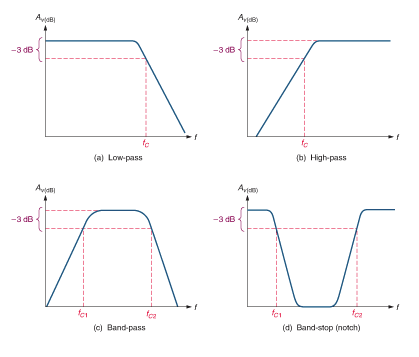
\includegraphics[scale=0.6]{Imagens/types.png}
  
  \label{fig:tipos}
  \small Fonte: www.dreamitdesignitbuildit.wordpress.com.
\end{figure}

Uma segunda classificação para os filtros é relacionada ao \textit{ripple} e a defasagem da resposta em frequência. Os tipos mais comuns empregados na prática são:

\begin{itemize}
    \item \textbf{Butterworth};
    \item \textbf{Chebyshev (tipo I ou II)};
    \item \textbf{Bessel}.
\end{itemize}

A figura \ref{fig:tipos2} mostra as características da resposta em frequência 
para os filtros citados acima.

\begin{figure}
  \centering
  \caption{Características dos filtros Butterworth, Chebyshev, Bessel e 
  Elíptico}
  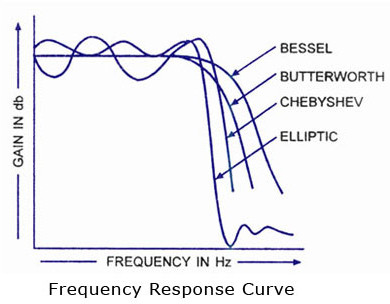
\includegraphics[scale=0.6]{Imagens/types2.jpg}
  
  \label{fig:tipos2}
  \small Fonte: http://www.circuitstoday.com
\end{figure}

\subsection{Frequência de Corte e Largura de Banda}
A frequência de corte ($f_c$ é a frequência para qual o filtro apresentará uma atenuação de 3dB e é o parâmetro fundamental para o projeto de filtros.
Outro parâmetro importante para os filtros do tipo passa-faixa e rejeita-faixa é a largura da banda de passagem, a qual é composta por uma frequência de corte inferior (denominada $f_1$) e uma superior ($f_2$).